\documentclass[tikz,border=5pt]{standalone}
\usepackage{tkz-euclide}
\usepackage{newtxmath}
\begin{document}
\tkzSetUpLabel[font=\scriptsize]
\tkzSetUpLine[semithick]
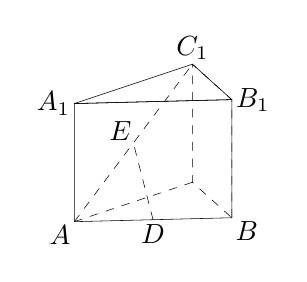
\begin{tikzpicture}
    \tkzDefPoints{0/0/A,2/.05/B,1.5/.5/C}
    \tkzDefPoints{0/1.5/A1,2/1.55/B1,1.5/2/C1}
    \tkzDrawPolygons(A1,B1,C1 A,B,B1,A1)
    \tkzDrawPolygons[dashed](B,B1,C1,C)
    \tkzDefMidPoint(A,B) \tkzGetPoint{D}
    \tkzDefMidPoint(A,C1) \tkzGetPoint{E}
    \tkzDrawSegments[dashed](A,C1 A,C D,E)
    \tkzLabelPoints[below left=-3pt](A)
    \tkzLabelPoints[below right=-3pt](B)
    \tkzLabelPoints[below=-1.75pt](D)
    \tkzLabelPoints[above left=-4pt](E)
    \tkzLabelPoint[above=-2pt](C1){$C_1$}
    \tkzLabelPoint[left=-2pt](A1){$A_1$}
    \tkzLabelPoint[right=-2pt](B1){$B_1$}
\end{tikzpicture}
\end{document}